Afin de comprendre comment se déroule la création d'une partie, nous avons réalisé deux diagrammes.

Le premier, un diagramme de cas d'utilisation, nous permet d'illustrer les actions que le joueur est autorisé à faire lorsqu'il lance le jeu et choisit la partie à laquelle il veut jouer.
\begin{figure}[!h]
\centering
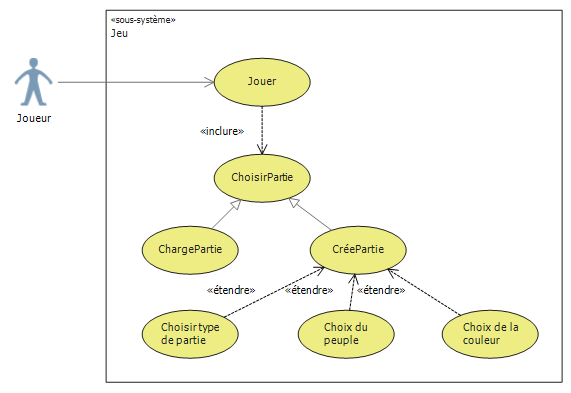
\includegraphics[width=\textwidth]{Parties/Images/cdu_CreationPartie.png}
\caption{Diagramme de cas d'utilisation : création d'une partie}
\label{fig:cdu_CreationPartie}
\end{figure}

\newpage
Ensuite nous avons créé un diagramme de séquence afin de déterminer la hiérarchie de création des différents éléments du jeu.
\begin{figure}[!h]
\centering
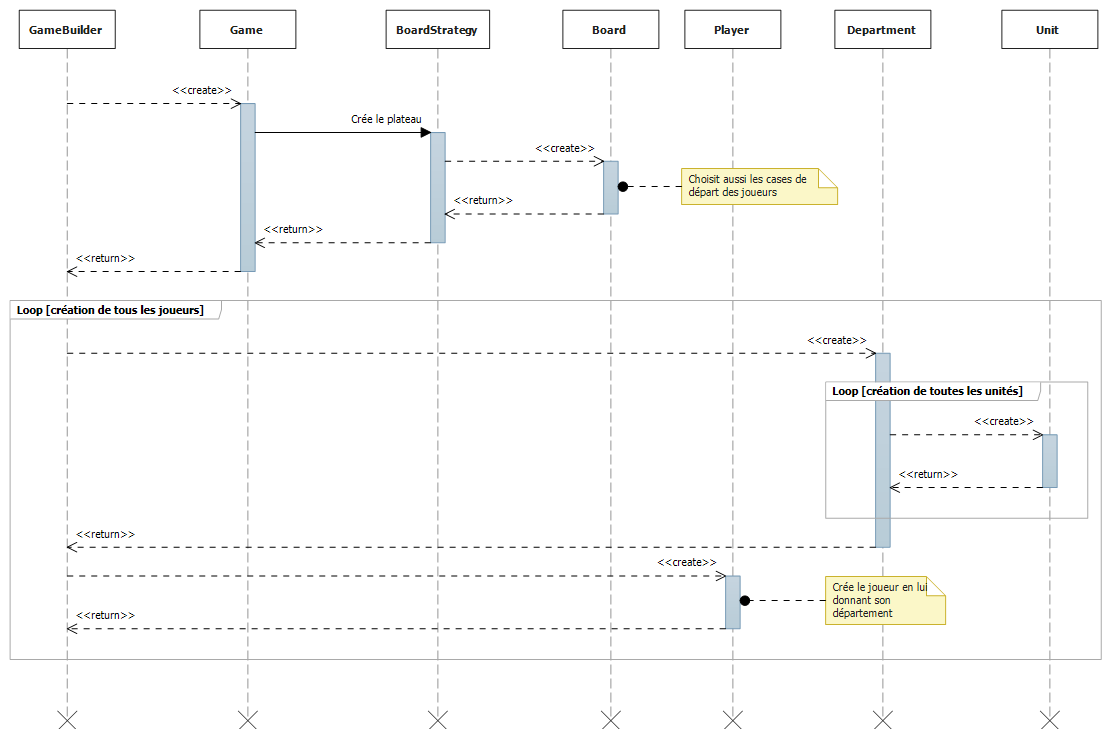
\includegraphics[width=\textwidth]{Parties/Images/seq_CreationPartie.png}
\caption{Diagramme de séquence : création d'une partie}
\label{fig:seq_CreationPartie}
\end{figure}
